\subsubsection{Impact of Graph Models}
\label{sec:models}

%\begin{figure}[thbp]
%\begin{center}
%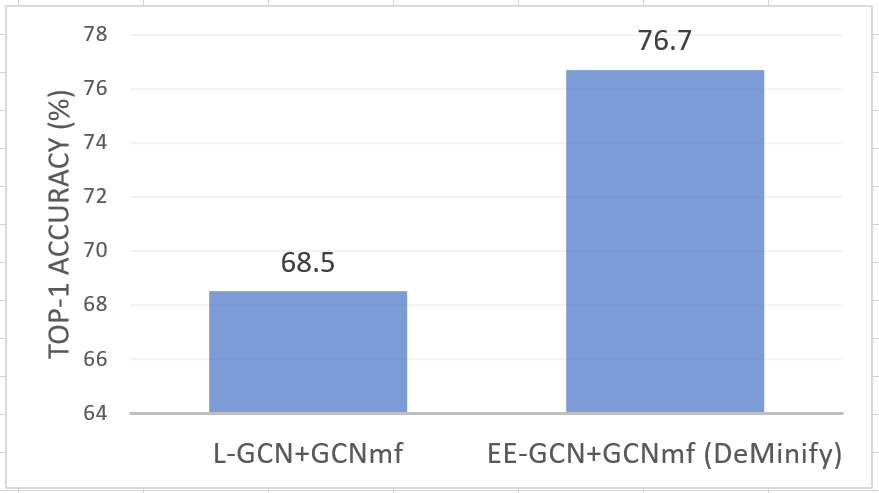
\includegraphics[width=2.6in]{figures/sensi-models-name}
%\vspace{-8pt}
%\caption{RQ3. Impact of Graph Model on Variable Name Prediction}
%\label{models-name-result}
%{\bf L-GCN}: Label Graph Convolutional Network, {\bf EE-GCN}: Edge-Enhanced Graph Convolutional Network, {\bf GCNmf}: Graph Convolutional Network - Missing Features
%\end{center}
%\end{figure}

%\begin{figure}[thbp]
%\begin{center}
%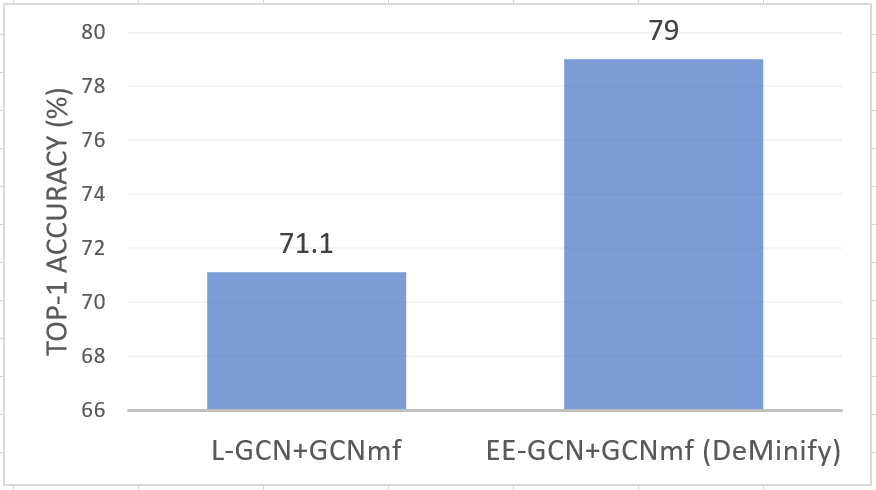
\includegraphics[width=2.6in]{figures/sensi-models-type}
%\vspace{-8pt}
%\caption{RQ3. Impact of Graph Model on Variable Type Prediction}
%\label{models-type-result}
%{\bf L-GCN}: Label Graph Convolutional Network, {\bf EE-GCN}: Edge-Enhanced Graph Convolutional Network, {\bf GCNmf}: Graph Convolutional Network - Missing Features
%\end{center}
%\end{figure}

\begin{table}[!ht]
  \centering
  \tabcolsep 2.5pt
    \begin{tabular}{|l|l|l|}
    \hline
        Accuracy (\%) & Name Prediction & Type Prediction\\ \hline
        Label-GCN+GCNmf & 68.5 & 71.1 \\ \hline
        EE-GCN+GCNmf (DeMinify) & 76.7 & 79 \\ \hline
    \end{tabular}
    {\bf Label-GCN}: Label Graph Convolutional Network, {\bf EE-GCN}: Edge-Enhanced Graph Convolutional Network, {\bf GCNmf}: Graph Convolutional Network - Missing Features
    \caption{Impact of EE-GCN on Accuracy}
    \label{tab:sensi-graph}
\end{table}

Table~\ref{tab:sensi-graph} shows the accuracies of the variant model
as we replaced the graph neural network EE-GCN with the Label Graph
Convolutional Network (Label-GCN)~\cite{label-gcn}. We did not replace
GCNmf because it is the core component in our solution, which
formulates the name/type recovery as the prediction of missing
features. As seen, Edge-Enhanced GCN helps improve accuracy more than
Label-GCN. EE-GCN enables the modeling of different types of edges
because it handles different edge types in different channels, while
Label-GCN just integrates the edge information as simple labels.
This is crucial for our problem in which the type dependencies
and the variable relations are well captured.


%2. EEGCN is a more advanced model by representing the edge in $N$ channels instead of a simple label compared with label-GCN (EEGCN+GCNmf+RG compared with LGCN+GCNmf+RG on both two tables)
